\subsection{Elastic bounce}
\label{sss:aquagpusph:boundaries:elasticbounce}
%
This is the simplest way to impose the boundary conditions, based on particle elastic bound within the wall, where
a elastic factor is applied in order to set plasticity.\\
%
In figure \ref{fig:aquagpusph:BounceScheme} a scheme of the elastic bound effect is shown. In \NAME walls are
defined by a set of vertexes (black balls), that have a normal\footnote{Ensure yourself that the provided normals
are normalized, \NAME will accept it as set by user} and area associated (area is stored on mass array).
In order to \NAME identify particles as vertexes, $imove$ flag must be set lower than 0.\\
%
Elastic bounce is applied when a particle will moved nearer to a vertex than `BoundDist' parameter introduced on
chapter \ref{sss:XML:SPH}, then the normal component of velocity is modified in order to get an elastic bound
multiplied by elastic factor `BoundElasticFactor'. If the elastic factor is 1, a fully elastic bound will
performed, however if elastic factor is 0, particle will stopped (normal component of the velocity will affected
only), so with values between 0 and 1 a semi-elastic bound will performed. You can set elastic factors out of
[0,1] bounds if you know what are you doing.\\
%
Main advantage of this boundary is the simplicity that reverts on a good performance, but using the Elastic bounce
boundary condition alone will return poor physics results, The Elastic bounce boundary condition is then aimed to
work with other boundary conditions, serving a second barrier for particles that can try to trespass the walls.
%
\begin{figure}[h!]
  \centering
  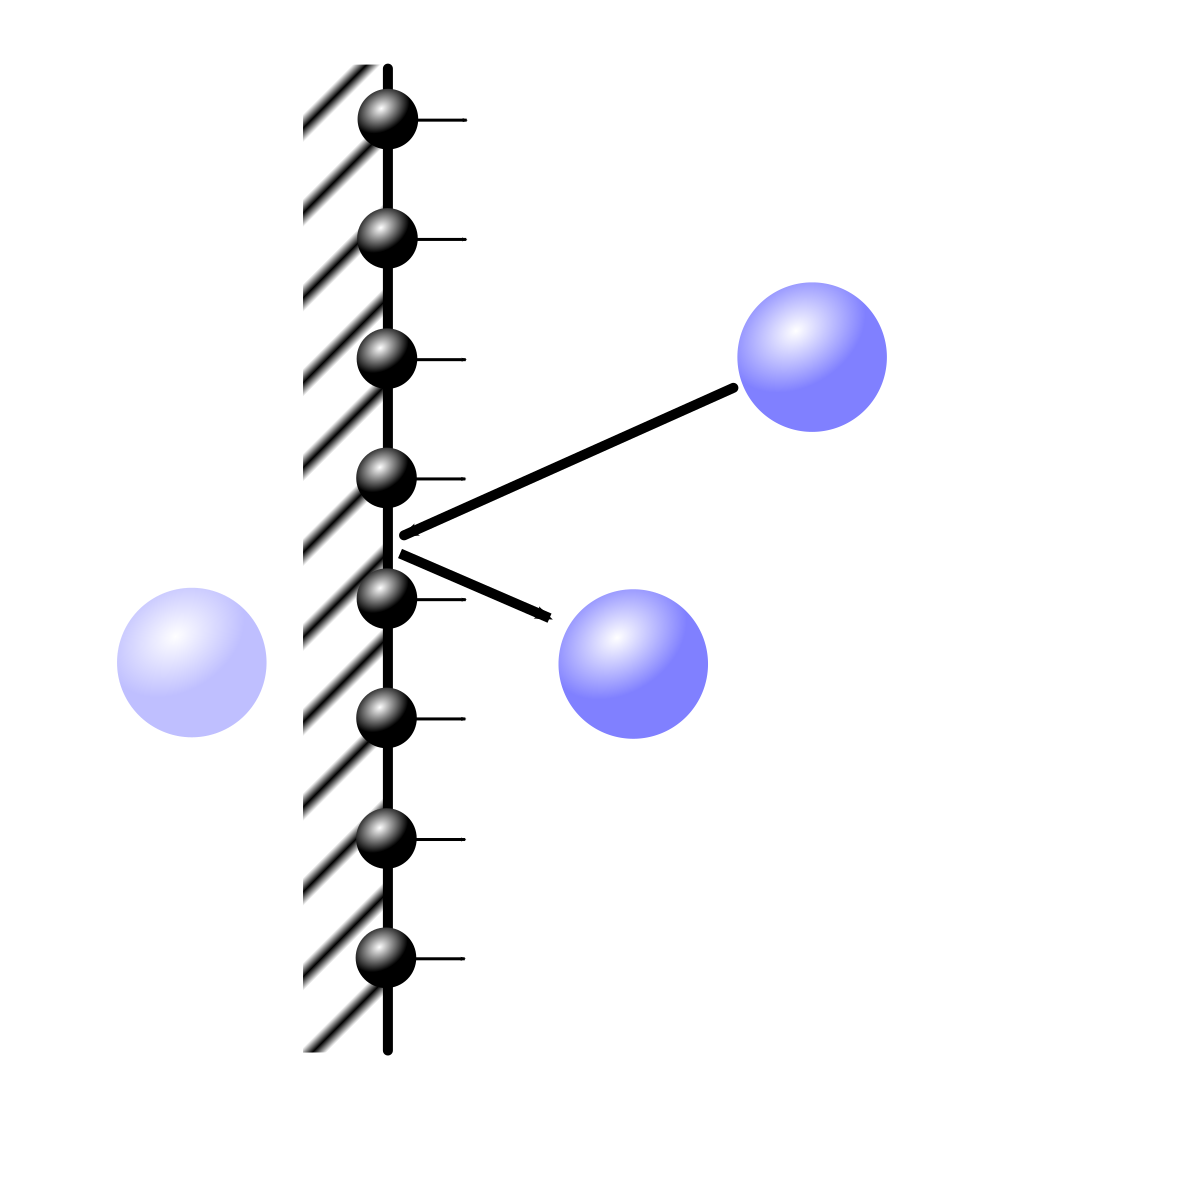
\includegraphics[width=0.25\textwidth]{ElasticBounce}
  \caption{Elastic bounce boundary scheme}
  \label{fig:aquagpusph:BounceScheme}
\end{figure}
%